\documentclass{amsart}
\usepackage{graphicx}
\graphicspath{{./}}
\usepackage{hyperref}
\usepackage{csvsimple}
\usepackage{longtable}
\usepackage{lscape}
\usepackage{epigraph}
\title{Why are Straightforward Measurements Sometimes Superior to Heavy Theory in Science?} 
\author{Zulfikar Moinuddin Ahmed}
\date{\today}
\begin{document}
\maketitle

\section{What is Scientific Theory}

All the noise and glory of Heaven and Earth are features of an inscrutible order, and Science is the pursuit of having certain knowledge of what drives this World, the world full of colour and magic, of joy and sorrow, of small things and large things.  Scientific viewpoint attempts to put order to all of this and find the universal laws of how all of this actually works.

Theories exist as stories of how the world works, some of them are scientific theories and others not.  For example the myth of Hellenistic Deity Apollo or Dionysus are theories too.  I have faith that my Soul is that of an Archangel of Heaven.  This can be seen as a theory that I believe is true.  These two examples are theories that are not scientific.  

Only some specific theories are scientific.  Scientific theories are restricted set of theories about the objective universe that attempt to explain and predict certain phenomena.  It is important to understand the limited scope of scientific theories.  They do not pretend to answer all possible question that can occur to anyone. They focus attention on a subset of phenomena and explain them by establishing them {\em against the background of actual measurements in the world}.  In other words, when theory $T$ predicts some outcome $A$ and this outcome is then found to be violated by measurements, then theory $T$ cannot be considered strictly speaking a valid scientific theory, regardless of the effort that went into producing it.  Scientific theories are those theories that are logically coherent and free of self-contradictions, and also match measurements on their domain of interest to adequate levels.  Without check against empirical measurements, theories are not scientific.

Sometimes heavy theory is simply not checked against measurements or they are too complex to have possibility of validation against thousands of experiments and measurements that have never been performed.  In those cases, {\em phenomenological theories} based on observations and measurements are going to be superior {\em scientific theories} than the complex alternatives that are heavy theory.

Now they might be superior in other ways; but they will be inferior as scientific theories. 

\section{Complex Racial Theories are Refuted by World Values Surveys Measurements}

From seventeenth to twentieth centuries in Europe, racial theories had formed and gained prominence.  I won't go into their content except to show how I refuted them all as scientific theories by inference from World Values Survey Data.  Here there are several related themes.  The major issues are that (a) are White people a different 'race' than others?  (b)  Are White people morally and intellectually and in other ways {\em superior} to others on Earth?

My discoveries from large sample high quality data from World Values Survey Wave 7 show that (a) and (b) can both be safely rejected as there is scant evidence that White people are significantly different enough from non-whites to be a separate 'race'; and there is little evidence that moral values of white people are significantly different from others.  These elementary exercises tell you that racial superiority theories had no scientific merit.

\section{Return To Elementary Questions}

I graduated magna cum laude from Princeton with a mathematics degree in 1995. For me talking about electrons are clear.  I know what an electron is.  I also am a humanities student.  Now how will we address the question of what a human being is?  I want to think here like a fifth grader.  I am 48 and for the past decade I was living with my aunt in Allen Texas not earning anything except disability, and so I have not been very social.  I have had many friends in the past but I do not think that it is possible to know 1000 people very well.  So what is a human being?  Most of us do not know enough personally to be able to answer by their own experience.  Member of the homo sapiens with DNA characterised by such and such.  That's fine.  Why should I accept any theory of racial difference?  I looked into this and the index of fixation is less than 0.12 across the globe.  There is scant evidence for multiple races with small variation in genes.

Now let's ask:  do people have differences in the way we have our convictions about whether its right or wrong not to pay the fare for public transport.


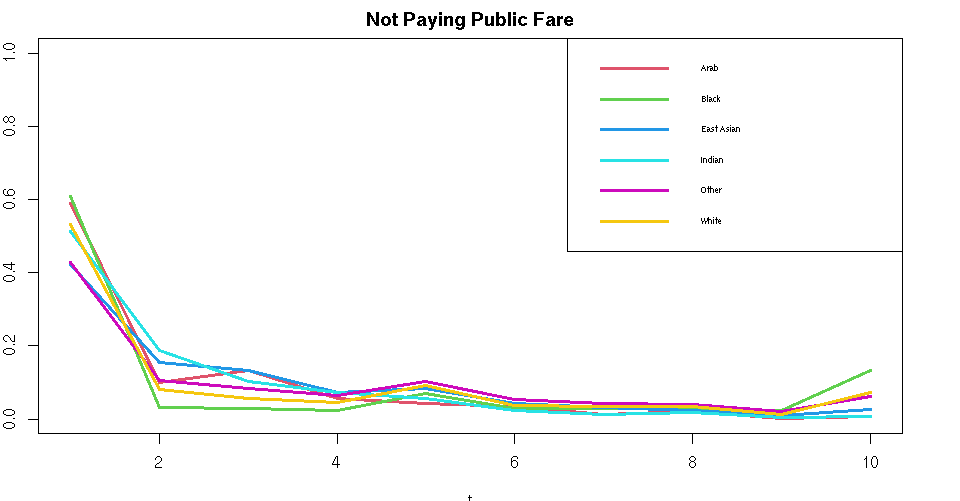
\includegraphics[scale=0.4]{public_fare.png}

Take a distance from the page and you will appreciate immediately that all the curves are actually quite close to each other.  Even without precise quantification, you can infer that there is not much difference between the convictions regarding paying public fare across different ethnicities across the world.

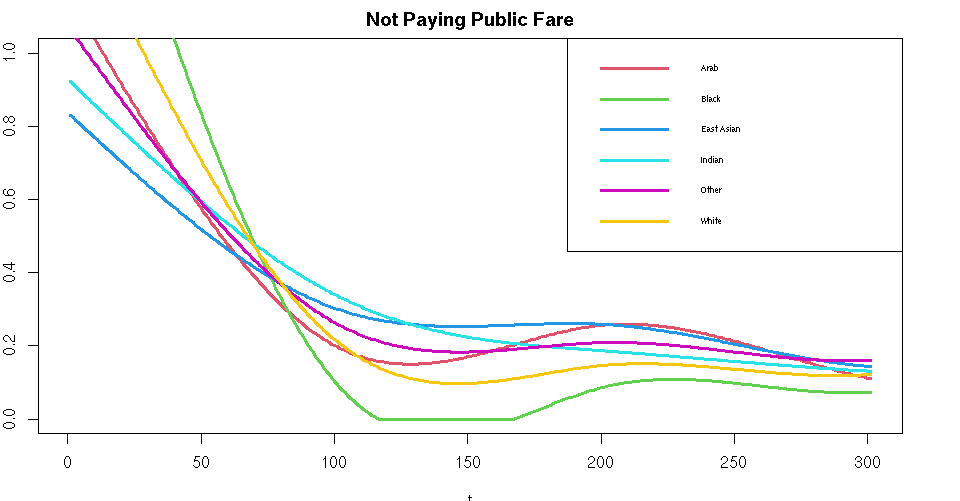
\includegraphics[scale=0.4]{public_fare_ghd.png}

Here you see Barndorff-Nielsen distribution fits of the same data, and you see some variation here but still you can assess visually that all ethnicities have minor differences in their convictions regarding paying public fares.

\section{Ethnicities are genetically and morally quite Uniform}

The above rough assessment I bring out to establish an important scientific principle, that the Human Race are genetically and morally as well quite homogeneous across the globe.  I will establish this as a {\em scientific theory} by elementary means.  

Now this is an interesting exercise, since people have claimed other sorts of theories focusing on racial differences in the past.  I will claim that my theory is the superior scientific theory and all these other theories are scientifically deficient.  This is an interesting issue, because it may be that racial theories are more {\em popular among the masses}.  But even if their appeal and popularity reach total consensus, they will be scientifically deficient. And this is important in Science.  We don't care about popularity of theories but about whether they are truth of nature or not.

\section{Human Race is Extremely Homogeneous in Moral Values}

There is a subtlety here that is conceptually difficult for people to understand.  There is no characteristic or moral value where people of one ethnicity or continental group distinguishes itself from the people of another group.  To make this conceptually clear, let's say for a given moral question, there are 'good people' and 'bad people' where good people mark one part say 1-5 and bad people mark 6-10.  In this situation strong homogeneity means that the proportion of good people in first ethnicity is roughly equal to proportion of good people in the second and respectively for bad people.

This is subtle today because there have been several centuries of indoctrination on the false theories of racial superiority.  Data from World Values Survey overwhelmingly disagrees with these sorts of racial ideas about morality.  White morality is roughly exactly the same as the morality of all other ethnicities and does not differ much from them.

\section{A Few Other Plots}

Is stealing justified?

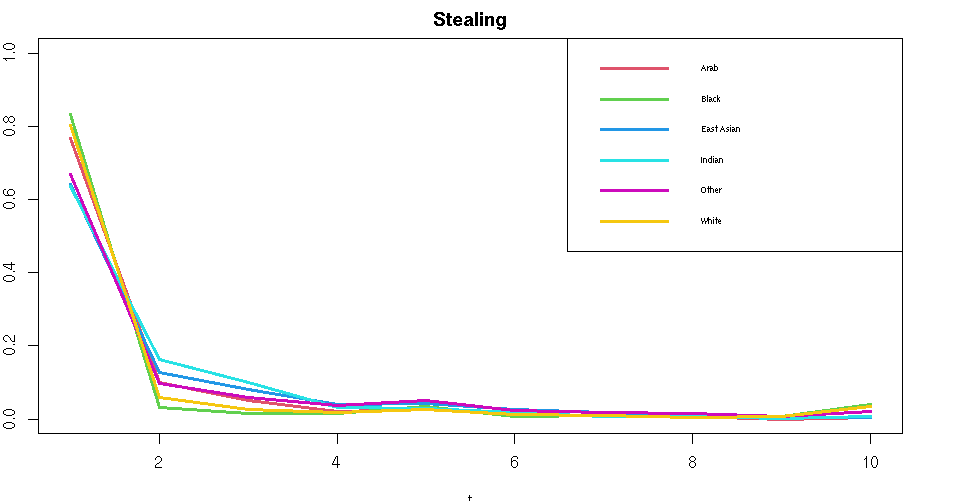
\includegraphics[scale=0.4]{jstealing.png}

Look at the graph from a distance and you will immediately realise that the difference from the mean is too tiny to make any great theories of moral difference by ethnicity.  You could spend your entire life doing something like this but you will be swept away by the overwhelming homogeneity of moral human nature and its universality.  The other moral graphs look similar and I have done more detailed analysis in earlier notes.  My 'Human Beings are Morally Homogeneous' theory will overwhelm any racial difference theory easily because the data is so clear that it will become quickly clear to any honest appraisal that these theorists have been fitting noise.

\section{A Last Example}

Consider convictions regarding prostitution.

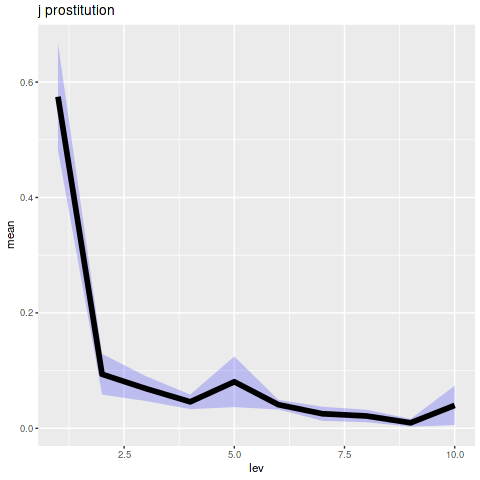
\includegraphics[scale=0.5]{jprost.png}

Now let's fit these with Barndorff-Nielsen distributions.

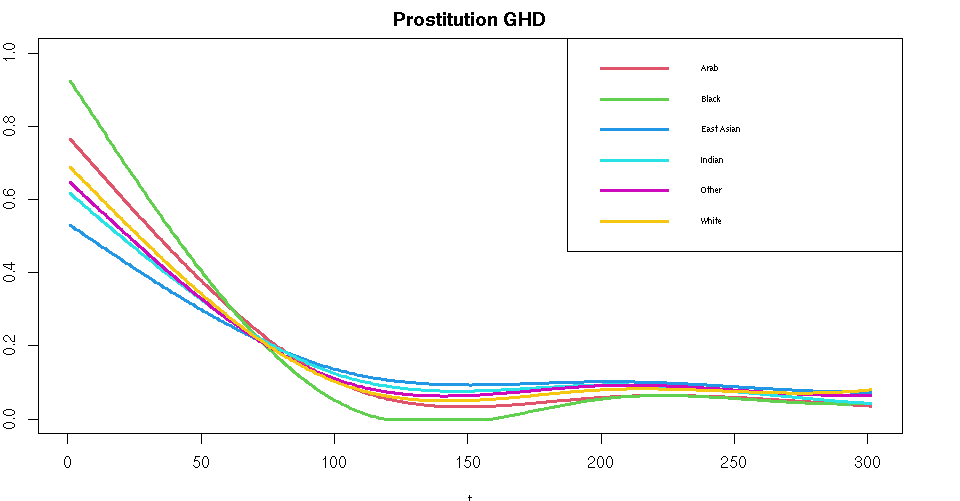
\includegraphics[scale=0.5]{jprost_ghd.png}

The differences follow the mean with extremely minor variation.  The Human Nature Moral Homogeneity totally dominates ethnic effects.

I leave it as an exercise to the reader to work through the impossibility of any racial theories of morality to face this homogeneity.  This is real science.  Racial theories are noise.


\end{document}